\section{Problem 1: EDGE DETECTION}\label{problem-1-edge-detection}
In this problem, please design several edge detection algorithms to satisfy the following requirements.

\subsection{(a)}\label{1_a}
Given an image, \nameref{sample1}.

Original image \nameref{sample1} for question \nameref{1_a}.
\begin{figure}
    \centering
    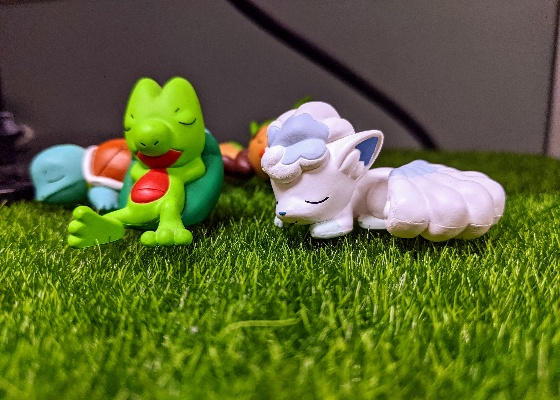
\includegraphics[width=0.7\textwidth]{hw2_sample_images/sample1.jpg}
    \caption{\textbf{sample1.jpg}}
    \label{sample1}
\end{figure}

\subsubsection{(1)}
Perform $1^{\mbox{st}}$ order edge detection and output the edge maps as \nameref{sample1}.

\paragraph{Motivation}
From the $1^{\mbox{st}}$ order derivative, we could observe the difference within the nearest points. Use non-parametric approaches to conduct edge detection.

\paragraph{Approach}
We could follow the steps of discrete case orthogonal gradient in \textit{Lec 3 page 12 -- 17}.
\begin{enumerate}
    \item Design the mask/filter. I have implemented \textit{n-point} with \(3, 4, 9\) in \textit{Lec 3 page 12, 14, 15}.
    \item Calculate \textbf{magnitudes/gradients} by convolution/weighted average \\
    with \texttt{scipy.signal.convolve2d}.
    \item Draw the histogram of magnitudes/gradients.
    \item Deciside the threshold by observing histogram.
\end{enumerate}

\paragraph{Performance of results}
In the end, I choose \textbf{9-point} with \textbf{\(k=2\)}, i.e. \textit{Sobel Mask} as my mask. And give the threshold as \textbf{\(25\)} according to  \nameref{prob1a1}.
\begin{figure}
    \centering
    \includegraphics[width=0.6\textwidth]{hw2_sample_images/tmp/prob1a1.png}
    \caption{\textbf{result1.jpg} Histogram of magnitudes}
    \label{prob1a1}
\end{figure}

Result of problem 1(a)(1): \nameref{result1}.
\begin{figure}
    \centering
    \includegraphics[width=0.7\textwidth]{hw2_sample_images/result1.jpg}
    \caption{\textbf{result1.jpg} $1^{\mbox{st}}$ order edge detection}
    \label{result1}
\end{figure}

\paragraph{Discussion}
For checking my approach is right or not, I also observe the \textbf{column} and \textbf{row} magnitudes in intermediates: \nameref{result1_col} \& \nameref{result1_row}.
\begin{figure}
    \centering
    \includegraphics[width=0.5\textwidth]{hw2_sample_images/tmp/result1_col.jpg}
    \caption{\textbf{result1.jpg} Column magnitudes}
    \label{result1_col}
\end{figure}

\begin{figure}
    \centering
    \includegraphics[width=0.5\textwidth]{hw2_sample_images/tmp/result1_row.jpg}
    \caption{\textbf{result1.jpg} Row magnitudes}
    \label{result1_row}
\end{figure}

With a different threshold, I try \nameref{result1_T2} and find out we keep too many edges.
\begin{figure}
    \centering
    \includegraphics[width=0.5\textwidth]{hw2_sample_images/tmp/result1_T=2.jpg}
    \caption{\textbf{result1.jpg} with threshold $T=2$}
    \label{result1_T2}
\end{figure}

\subsubsection{(2)}
Perform $2^{\mbox{nd}}$ order edge detection and output the edge maps as \textbf{result2.jpg}.

\paragraph{Motivation}
We find out there is some tricky problem of deciding the threshold in $1^{st}$ order edge detection. So we could get the $2^{nd}$ order derivative to obtain the \alert{zero-crossing} points to support us.

\paragraph{Approach}
We could follow the steps of discrete approximation of Laplacian in \textit{Lec 3 page 26 -- 37}.
\begin{enumerate}
    \item Design the mask/filter. I have implemented \textit{n-neighbor} with \(4, 8\). For \textit{8-neighbor}, there are \textit{separable}, \textit{non-separable} and other mask array in \textit{Lec 3 page 29}.
    \item Compute \textbf{Laplacian} by convolution/weighted average with \texttt{scipy.signal.convolve2d}.
    \item Draw the histogram of magnitudes/gradients.
    \item Set up a threshold to separate \textbf{zero} and \textbf{non-zero} by observing histogram, output as $G\textnormal{\textquotesingle}$.
    \item For $G\textnormal{\textquotesingle}(j, k) = 0$, decide whether $(j, k)$ is a \textbf{zero-crossing} points by its \alert{8-neighbor} contains $-1$ \& $0$ simultaneously.
\end{enumerate}

\paragraph{Performance of results}
In the end, I choose \textbf{non-separable 8-nieghbor} as my mask. And give the threshold as \textbf{\(5\)} according to \nameref{prob1a2}.
\begin{figure}
    \centering
    \includegraphics[width=0.6\textwidth]{hw2_sample_images/tmp/prob1a2.png}
    \caption{\textbf{result2.jpg} Histogram of Laplacian}
    \label{prob1a2}
\end{figure}

Result of problem 1(a)(2): \nameref{result2}.
\begin{figure}
    \centering
    \includegraphics[width=0.7\textwidth]{hw2_sample_images/result2.jpg}
    \caption{\textbf{result2.jpg} $2^{\mbox{nd}}$ order edge detection}
    \label{result2}
\end{figure}

\paragraph{Discussion}
I try the different threshold to observe the variation \nameref{result2_T25} \& \nameref{result2_T50}.
\begin{figure}
    \centering
    \includegraphics[width=0.5\textwidth]{hw2_sample_images/tmp/result2_T25.jpg}
    \caption{\textbf{result2.jpg} Threshold $T=25$}
    \label{result2_T25}
\end{figure}

\begin{figure}
    \centering
    \includegraphics[width=0.5\textwidth]{hw2_sample_images/tmp/result2_T50.jpg}
    \caption{\textbf{result2.jpg} Threshold $T=50$}
    \label{result2_T50}
\end{figure}

\subsubsection{(3)}
Perform \textit{Canny} edge detection and output the edge maps as \textbf{result3.jpg}.

\paragraph{Motivation}
\textit{Canny} edge dector is famous methods. It has good detection, localization and single response constraint, i.e. the edge should be as \textbf{thin} as possible. Finally, its steps are simple to implement.

\paragraph{Approach}
We could follow the five-step of \textit{Canny} method in \textit{Lec 3 page 19 -- 23}.
\begin{enumerate}
    \item Noise reduction with \textbf{Gaussian filter} mask.
    \item Compute gradient magnitude and orientation by reusint $1^{st}$ order detection methods.
    \item Non-maximal suppression, follow the \nameref{non_max_suppr}, I split the \textbf{8-neighbor} of $G(j, k)$ as \alert{4 direction parts}. And according to the formula in \textit{Lec 3 page 21} to calculate $G_{N}(j, k)$.
    \item Hysteretic thresholding, label each pixels according to two threshold $T_{H}$ \& $T_{L}$. And obtain \alert{exact edge pixels} and \alert{candidate pixels}.
    \item Connected component labeling method, I implement \textbf{8-neighbor} methods that if the neighbor of candidate pixels contains \alert{any other} edge pixels \alert{or any other} candidate pixels. I'll return it as edge pixels.
\end{enumerate}
\begin{figure}
    \centering
    \includegraphics[width=0.4\textwidth]{hw2_sample_images/non_max_suppr.png}
    \caption{Illustration of non-maximal suppression}
    \label{non_max_suppr}
\end{figure}

\paragraph{Performance of results}
In the end, I choose $T_{H}=50$ \& $T_{L}=15$ after several tries.

Result of problem 1(a)(3): \nameref{result3}.
\begin{figure}
    \centering
    \includegraphics[width=0.7\textwidth]{hw2_sample_images/result3.jpg}
    \caption{\textbf{result3.jpg} Canny edge detection}
    \label{result3}
\end{figure}

\paragraph{Discussion}
I reveal the intermediates of Canny edges.
\begin{itemize}
    \item \nameref{result3_cannys1} Noise reduction 
    \item \nameref{result3_cannys2} Compute gradient magnitude and orientation
    \item \nameref{result3_cannys3} Non-maximal suppression
    \item \nameref{result3_cannys4} Hysteretic thresholding
\end{itemize}
\begin{figure}
    \centering
    \includegraphics[width=0.5\textwidth]{hw2_sample_images/tmp/result3_cannys1.jpg}
    \caption{\textbf{result3.jpg} Step1.}
    \label{result3_cannys1}
\end{figure}

\begin{figure}
    \centering
    \includegraphics[width=0.5\textwidth]{hw2_sample_images/tmp/result3_cannys2.jpg}
    \caption{\textbf{result3.jpg} Step2.}
    \label{result3_cannys2}
\end{figure}

\begin{figure}
    \centering
    \includegraphics[width=0.5\textwidth]{hw2_sample_images/tmp/result3_cannys3.jpg}
    \caption{\textbf{result3.jpg} Step3.}
    \label{result3_cannys3}
\end{figure}

\begin{figure}
    \centering
    \includegraphics[width=0.5\textwidth]{hw2_sample_images/tmp/result3_cannys4.jpg}
    \caption{\textbf{result3.jpg} Step4.}
    \label{result3_cannys4}
\end{figure}

\subsubsection{(4)}
Apply an edge crispening method to the given image, and output the result as \textbf{result4.jpg}. Please also generate an edge map of \textbf{result4.jpg} as \textbf{result5.jpg}.

\paragraph{For \textbf{result4.jpg}}
\paragraph{Motivation}
We could treat \text{edge} as \textbf{high frequency} and conduct \textbf{high-pass filtering}. But remember that, if there are some \textbf{noise} in the image, we also \textbf{amplify} the noise at the same time. So I try \textbf{Unsharp masking} first. It combine low-pass and all-pass to get better results.

\paragraph{Approach}
We could follow the unsharp masking and its combination in \textit{Lec 3 page 6}.
\begin{enumerate}
    \item Build low-pass filtering matrix. Reuse homework 1.
    \item Compute low-pass result $F_{L}(j, k)$ by convolution/weighted average \\
    with \texttt{scipy.signal.convolve2d}.
    \item Compute $G(j, k)$ by combining all-pass $F(j, k)$ and low-pass $F_{L}(j, k)$ with formula \cref{unsharp_mask}.
\end{enumerate}

\begin{equation} \label{unsharp_mask}
    G(j, k) = \frac{c}{2c-1}F(j, k)-\frac{1-c}{2c-1}F_{L}(j, k)
\end{equation}
where $\frac{3}{5} \leq c \leq \frac{5}{6}$

\paragraph{Performance of results}
In the end, I choose $c=\frac{3}{5}$ .

Result of problem 1(a)(4): \nameref{result4}.
\begin{figure}
    \centering
    \includegraphics[width=0.7\textwidth]{hw2_sample_images/result4.jpg}
    \caption{\textbf{result4.jpg} Edge crispening}
    \label{result4}
\end{figure}

\paragraph{Discussion}
For different parameters $c$, \alert{to do...}

\paragraph{For \textbf{result5.jpg}}
\paragraph{Approach}
I use \textbf{Canny edge detection} on \nameref{result4}.

\paragraph{Performance of results}
In the end, I keep $T_{H}=50$ \& $T_{L}=15$ as the former.

Result of problem 1(a)(4): \nameref{result5}.
\begin{figure}
    \centering
    \includegraphics[width=0.7\textwidth]{hw2_sample_images/result5.jpg}
    \caption{\textbf{result5.jpg} Edge crispening}
    \label{result5}
\end{figure}

\subsubsection{(5)}
Compare \textbf{result1.jpg}, \textbf{result2.jpg}, \textbf{result3.jpg} and \textbf{result5.jpg}. Provide some discussions and findings in the report.

\paragraph{From $1^{st}$ order to $2^{nd}$ order}
In constrast to $1^{\mbox{st}}$ order edge detection \nameref{result1}, $2^{\mbox{nd}}$ order edge detection could sketch more \textbf{particulars}.
But we could see there some \textbf{dust} on the background in $2^{nd}$ order edge map.

Both of them we could observe the \textbf{histogram} of magnitudes and Laplacian respectively.

\paragraph{From $1^{st}$ \& $2^{nd}$ order to Canny}
I consider that it is difficult of choosing $T_{H}$ \& $T_{L}$. But in contrast to $1^{\mbox{st}}$ and $2^{\mbox{nd}}$ order edge detection, Canny edge detection is good methods that it is \textbf{common/reasonable(?) edge map} for me.

\paragraph{Edge crispening than Canny}
It is interesting that we could get more \alert{details} after \textbf{edge crispening}. We could see the \textit{streamline over the river}. But it makes me fear too intensive.

\paragraph{Conclusion of Problem 1 (a)}
The tricky points of \textbf{edge detection} is choose a \alert{good threshold} that keep/remove points to construct edge.

And it seems ``NO FREE LAUNCH''. If we want to use \textbf{Canny detection} to get better results, we need to carefully check parameters. The future work may design the mechanism of choosing threshold automatically by different user preference.

\subsection{(b)}\label{1_b}
Please design an algorithm to obtain the edge map of \nameref{sample2} as best as you can. Describe the steps in detail and provide some discussions.

Original image \nameref{sample2} for question \nameref{1_b}.
\begin{figure}
    \centering
    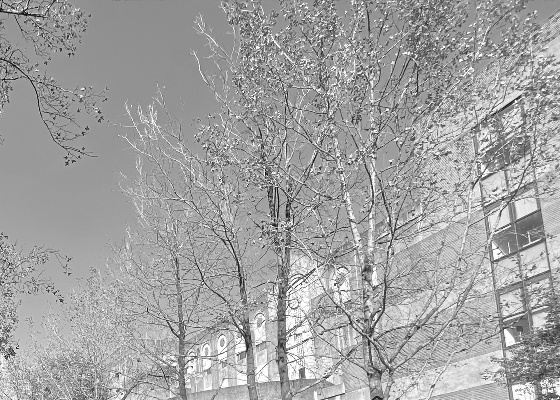
\includegraphics[width=0.7\textwidth]{hw2_sample_images/sample2.jpg}
    \caption{\textbf{sample2.jpg}}
    \label{sample2}
\end{figure}

\paragraph{Motivation}
The difficulty of the problem is that the \nameref{sample2} is too bright. But if we \textbf{increase its contrast}. You could see some \textbf{dust pixel} start appearing \textit{on the sky around of buildings}.

So we should carefully design the \textbf{image enhancement} and \textbf{denoising} (if necessary) as \textbf{data preprocessing} then do \textbf{edge detection}.
% insert contrast result here!

\paragraph{Approach}
In the end, my approach is
\begin{enumerate}
    \item Use \alert{10 times} \textbf{low-pass filter} to denoise.
    \item Use \textbf{power law transformation} with $p=1.4$ to improve the contrast of \textbf{with region}, \textit{sky region}. \\
    Note: An amazing is that I make transformation on $(0, 255)$ \alert{instead} \textbf{normalization} on $(0, 1)$.
    \item Use \textbf{edge crispening} to make edge more clear.
    \item Use \textbf{Canny edge detection} with $T_{H} = 60$ \& $T_{L}= 30$ to get result.
\end{enumerate}

\paragraph{Performance of results}
Result of problem 1(b): \nameref{result1b}.
\begin{figure}
    \centering
    \includegraphics[width=0.7\textwidth]{hw2_sample_images/prob1b.jpg}
    \caption{Result of problem 1 (b)}
    \label{result1b}
\end{figure}

\paragraph{Discussion}
I think there are two key points:
\begin{itemize}
    \item Denoise to remove the \textbf{dust}. I consider that it is why we see the image with \textbf{veil}. So I choose \textbf{low-pass filtering}.
    \item The other one is make \textbf{really strong contrast} on buildings and sky.
\end{itemize}
Here is my intermediates, enjoy it! :-)
\begin{itemize}
    \item \nameref{prob1b_LP} 10-times low-pass filtering
    \item \nameref{prob1b_HC} Non-normalization of power-law transformation
    \item \nameref{prob1b_EC} Edge crispening
\end{itemize}
\begin{figure}
    \centering
    \includegraphics[width=0.5\textwidth]{hw2_sample_images/tmp/prob1b_LP.jpg}
    \caption{Problem 1 (b) Step1.}
    \label{prob1b_LP}
\end{figure}

\begin{figure}
    \centering
    \includegraphics[width=0.5\textwidth]{hw2_sample_images/tmp/prob1b_HC.jpg}
    \caption{Problem 1 (b) Step2.}
    \label{prob1b_HC}
\end{figure}

\begin{figure}
    \centering
    \includegraphics[width=0.5\textwidth]{hw2_sample_images/tmp/prob1b_EC.jpg}
    \caption{Problem 1 (b) Step3.}
    \label{prob1b_EC}
\end{figure}
